\documentclass[usenatbib]{mn2e}
\usepackage{amsmath} 
\usepackage{amssymb} 
\usepackage{graphics}
\usepackage{graphicx}
\usepackage{epsfig}  
\usepackage{morefloats}
\def\be{\begin{equation}}
\def\ee{\end{equation}}
\def\ba{\begin{eqnarray}}
\def\ea{\end{eqnarray}}

\newcommand{\documentname}{paper~}
\newcommand{\match}{{\tt match}~}
\newcommand{\apj}{ApJ}  
\newcommand{\apjs}{ApJS}  
\newcommand{\apjl}{ApJL}  
\newcommand{\aj}{AJ}  
\newcommand{\mnras}{MNRAS}  
\newcommand{\mnrassub}{MNRAS accepted}  
\newcommand{\aap}{A\&A}  
\newcommand{\aaps}{A\&AS}  
\newcommand{\araa}{ARA\&A}  
\newcommand{\nat}{Nature}  
\newcommand{\physrep}{PhR}
\newcommand{\pasp}{PASP}    
\newcommand{\pasj}{PASJ}    

\newcommand{\kms}{\,km~s$^{-1}$}
\def\squig{\sim\!\!}
\newcommand{\LCDM}{$\Lambda$CDM~}
\newcommand{\beq}{\begin{eqnarray}}  
\newcommand{\eeq}{\end{eqnarray}}   
\newcommand{\zz}{$z\sim 3$} 
\newcommand{\avg}[1]{\langle{#1}\rangle}  
\newcommand{\ly}{{\ifmmode{{\rm Ly}\alpha}\else{Ly$\alpha$~}\fi}}
\newcommand{\hMpc}{{\ifmmode{h^{-1}{\rm Mpc}}\else{$h^{-1}$Mpc }\fi}}  
\newcommand{\hGpc}{{\ifmmode{h^{-1}{\rm Gpc}}\else{$h^{-1}$Gpc }\fi}}  
\newcommand{\hmpc}{{\ifmmode{h^{-1}{\rm Mpc}}\else{$h^{-1}$Mpc }\fi}}  
\newcommand{\hkpc}{{\ifmmode{h^{-1}{\rm kpc}}\else{$h^{-1}$kpc }\fi}}  
\newcommand{\hMsun}{{\ifmmode{h^{-1}{\rm
        {M_{\odot}}}}\else{$h^{-1}{\rm{M_{\odot}}}$}\fi}}   
\newcommand{\hmsun}{{\ifmmode{h^{-1}{\rm
        {M_{\odot}}}}\else{$h^{-1}{\rm{M_{\odot}}}$}\fi}}   
\newcommand{\Msun}{{\ifmmode{{\rm {M_{\odot}}}}\else{${\rm{M_{\odot}}}$}\fi}}  
\newcommand{\msun}{{\ifmmode{{\rm {M_{\odot}}}}\else{${\rm{M_{\odot}}}$}\fi}}  
\newcommand{\lya}{{Lyman$\alpha$~}}
\newcommand{\clara}{{\texttt{CLARA}}~}
\newcommand{\rand}{{\ifmmode{{\mathcal{R}}}\else{${\mathcal{R}}$ }\fi}}  
\newcommand{\Lsun}{\mbox{\,$L_{\odot}$}}
\newcommand{\like}{\mathscr{L}}
\newcommand{\bftheta}{\mathbf{\Theta}}
\newcommand{\degree}{\ensuremath{^\circ}}
\def\spose#1{\hbox to 0pt{#1\hss}}
\def\simlt{\mathrel{\spose{\lower 3pt\hbox{$\mathchar"218$}}
     \raise 2.0pt\hbox{$\mathchar"13C$}}}
\def\simgt{\mathrel{\spose{\lower 3pt\hbox{$\mathchar"218$}}
     \raise 2.0pt\hbox{$\mathchar"13E$}}}
\font\smcap=cmcsc10

\begin{document}

\title[Quasar line profiles from  rest-frame UV to Optical]{Quasar line profiles from rest-frame UV to Optical}    
\author[P. Lira and J.E. Mejia-Restrepo]{
\parbox[t]{\textwidth}{\raggedright 
Paulina Lira $^{1}$ and
Juli\'an Mej\'ia-Restrepo$^{1}$ 
}
\vspace*{6pt}\\
$^{1}$ Departamento de Astronom\'{i}a, Universidad de Chile, Camino el
Observatorio 1515, Santiago, Chile} 

\maketitle

\begin{abstract}
 Quasar line profiles from  rest-frame UV to Optical 
\end{abstract}

\begin{keywords}
{galaxies: AGNs, quasars, Broad line region} 
\end{keywords}


\section{Plots}

\subsection{Continuous}

\begin{figure*}
\begin{center}
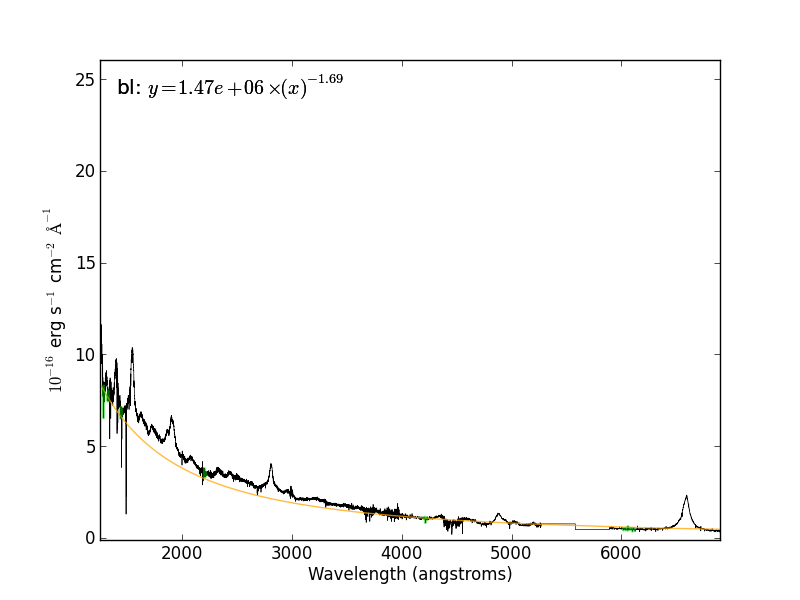
\includegraphics[width=0.49\linewidth,angle=0]{./full_range/continuous_0.png}
\vspace{5mm}
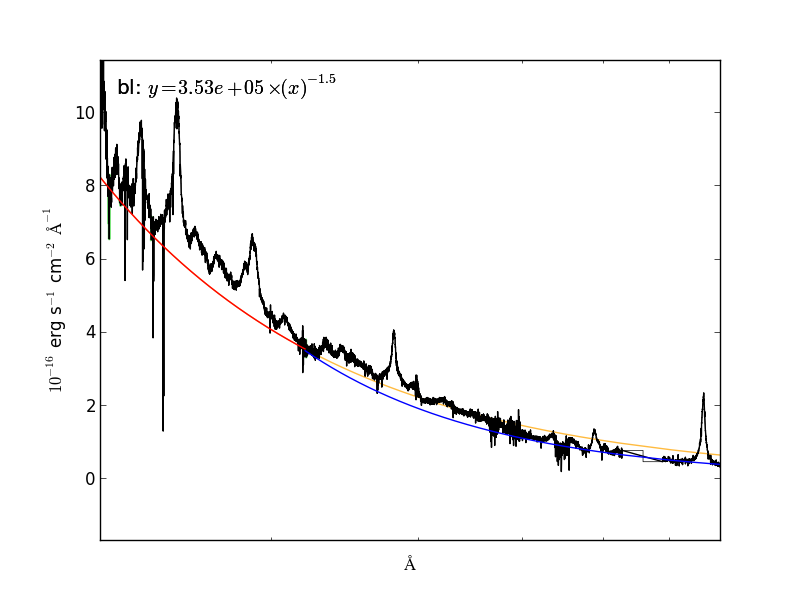
\includegraphics[width=0.46\linewidth,angle=0]{./Fe_fit_slope_break/break_continuous_0.png}\\
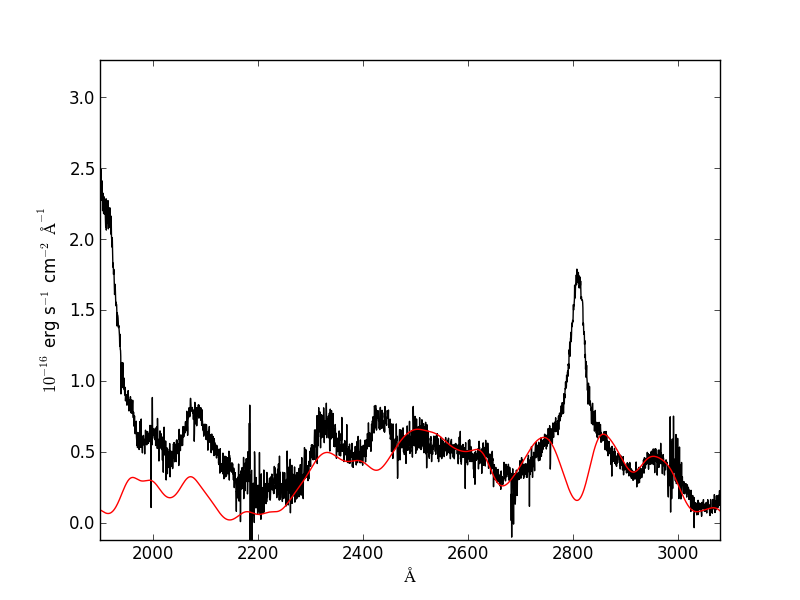
\includegraphics[width=0.49\linewidth,angle=0]{./full_range/fe_fit_SBB_0.png}
\hspace{5mm}
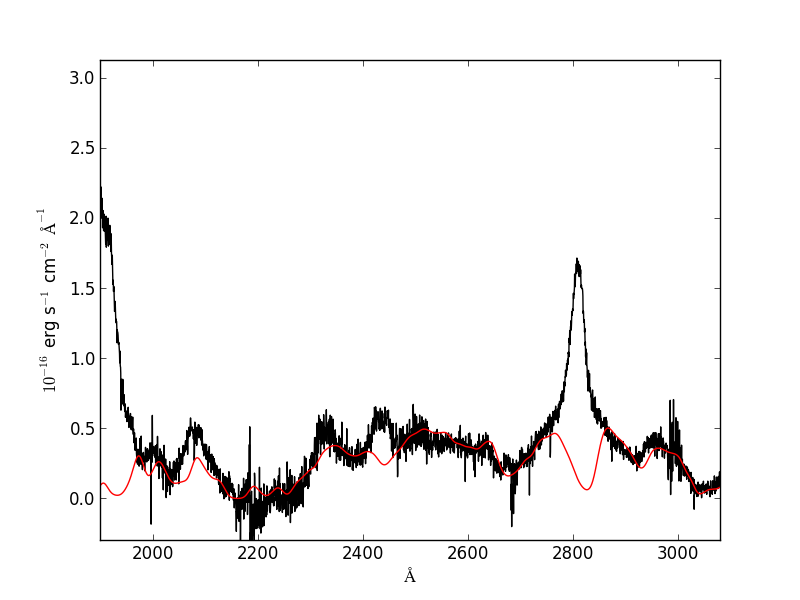
\includegraphics[width=0.46\linewidth,angle=0]{./Fe_fit_slope_break/fe_fit_SBB_0.png}\\
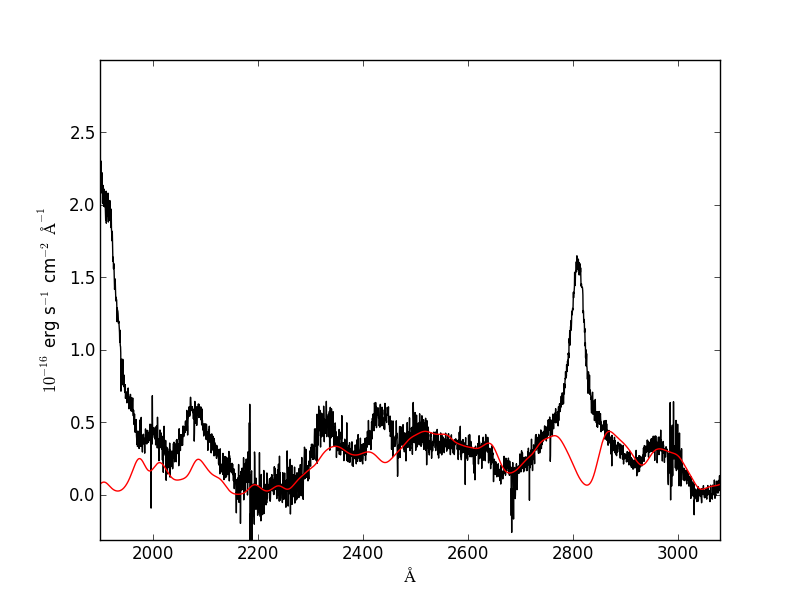
\includegraphics[width=0.46\linewidth,angle=0]{./Blue/fe_fit_SBB_0.png}
\vspace{5mm}
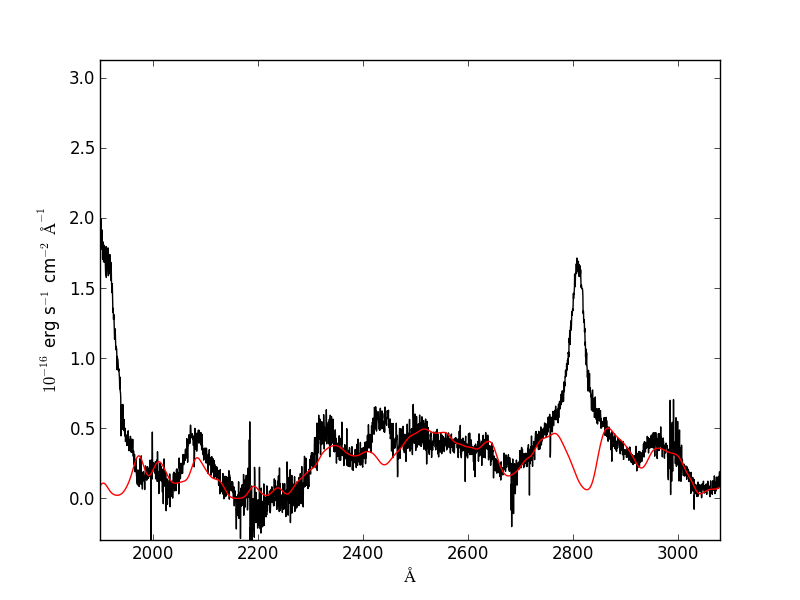
\includegraphics[width=0.49\linewidth,angle=0]{./red/fe_fit_SBB_0.png}\\

\end{center} 
\caption{J0155-1023 \label{fig:landscape}}   
\end{figure*}

\newpage


\begin{figure*}
\begin{center}
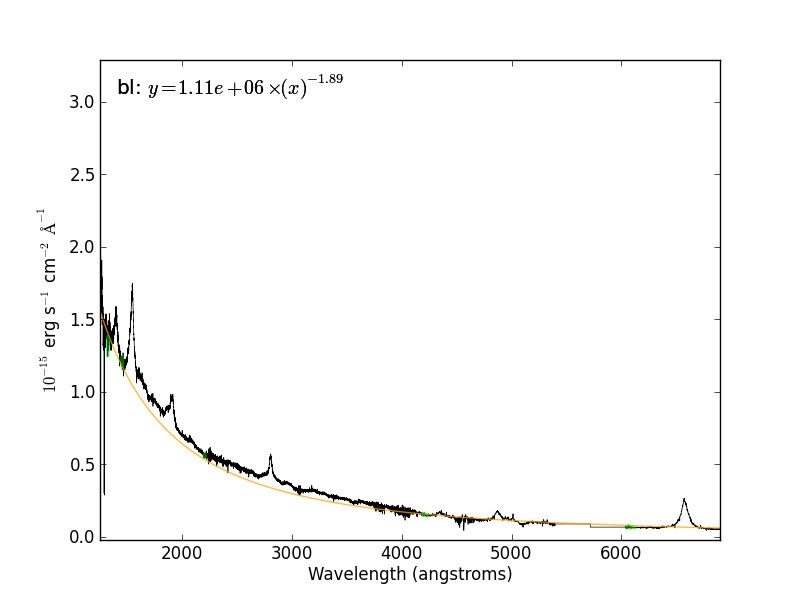
\includegraphics[width=0.49\linewidth,angle=0]{./full_range/continuous_1.png}
\vspace{5mm}
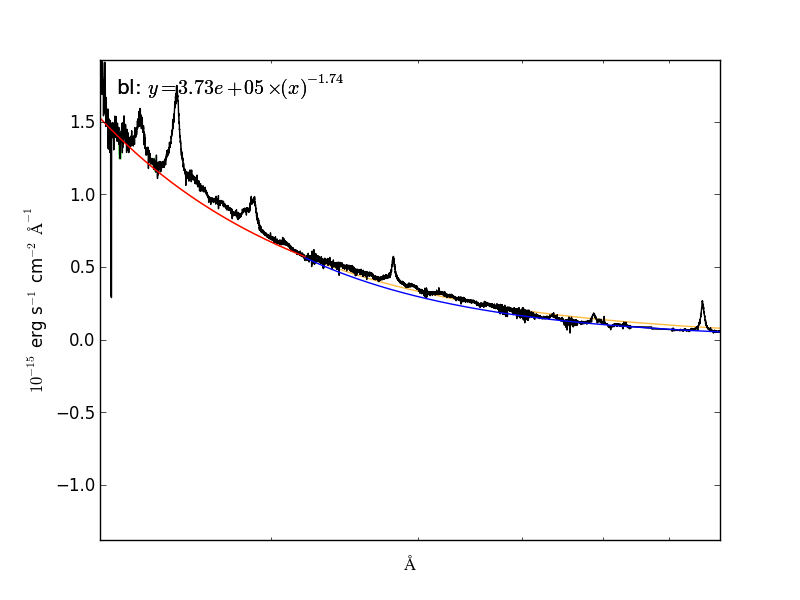
\includegraphics[width=0.46\linewidth,angle=0]{./Fe_fit_slope_break/break_continuous_1.png}\\
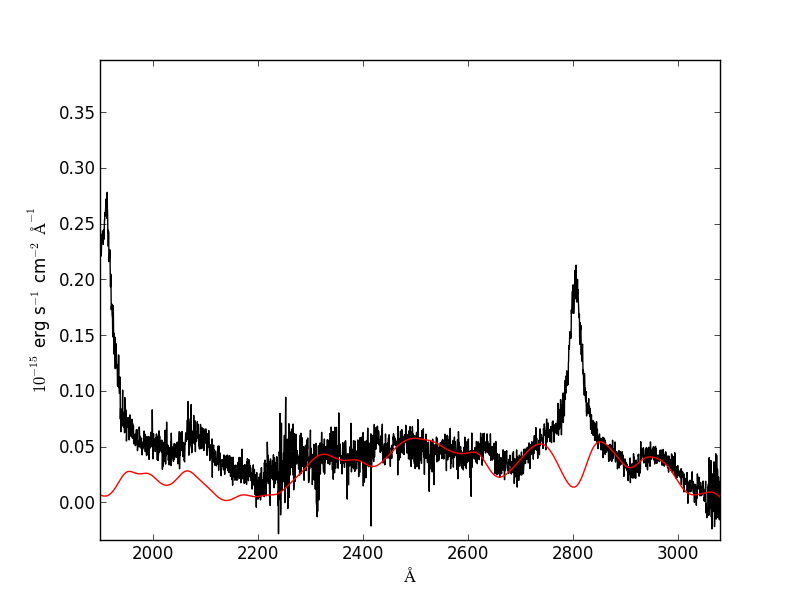
\includegraphics[width=0.49\linewidth,angle=0]{./full_range/fe_fit_SBB_1.png}
\hspace{5mm}
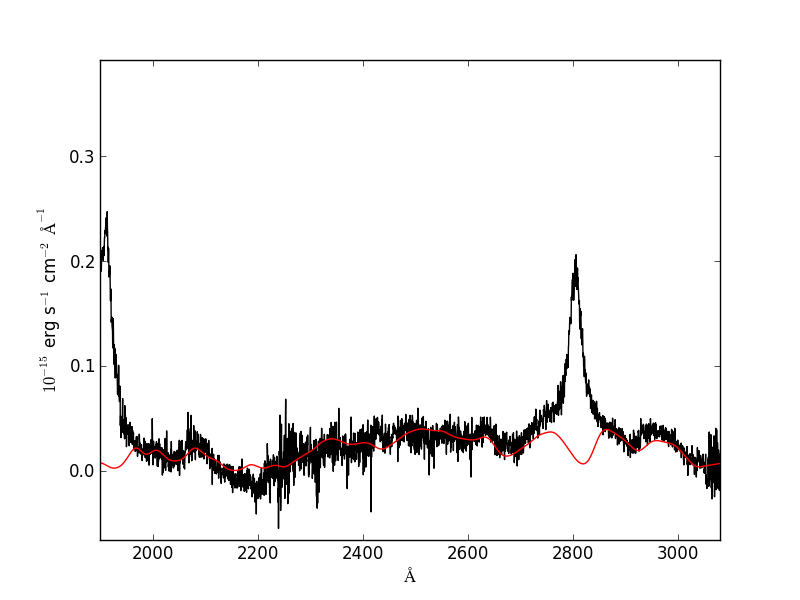
\includegraphics[width=0.46\linewidth,angle=0]{./Fe_fit_slope_break/fe_fit_SBB_1.png}\\
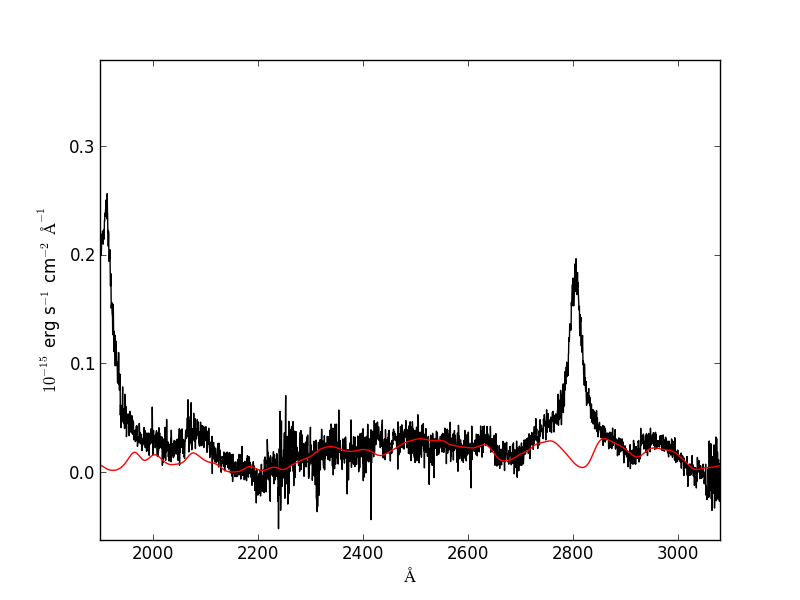
\includegraphics[width=0.46\linewidth,angle=0]{./Blue/fe_fit_SBB_1.png}
\vspace{5mm}
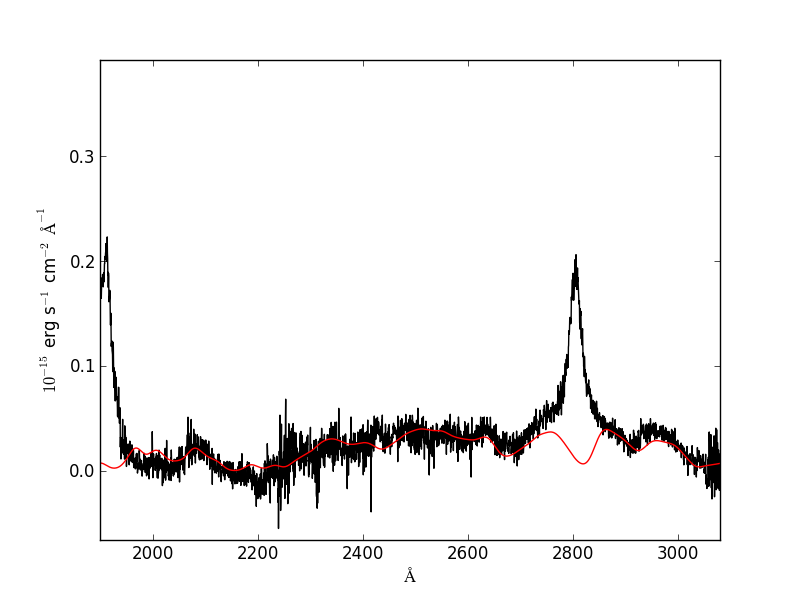
\includegraphics[width=0.49\linewidth,angle=0]{./red/fe_fit_SBB_1.png}\\

\end{center} 
\caption{J1152+0702 \label{fig:landscape}}   
\end{figure*}

\newpage

\begin{figure*}
\begin{center}
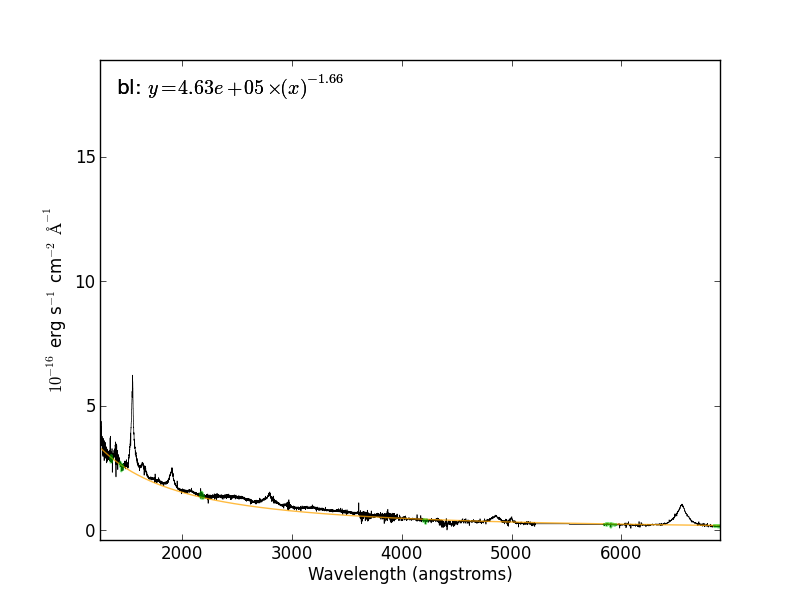
\includegraphics[width=0.49\linewidth,angle=0]{./full_range/continuous_2.png}
\vspace{5mm}
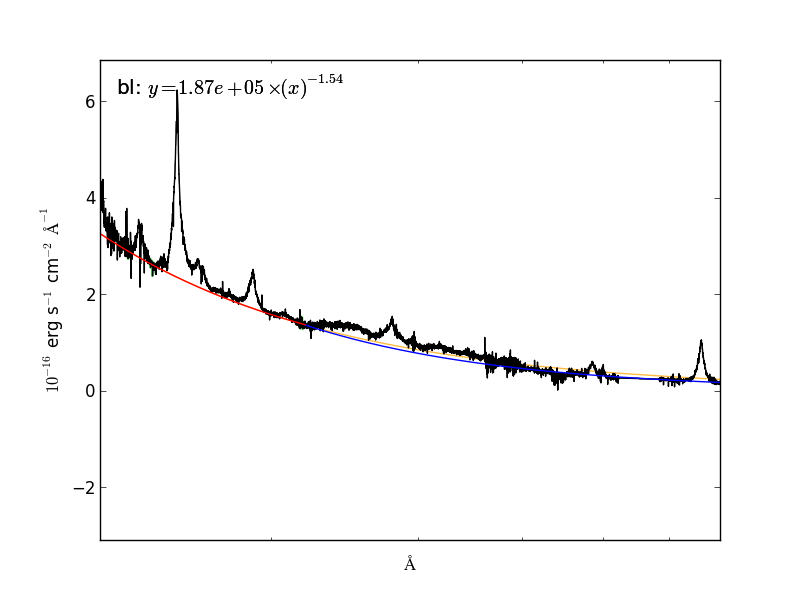
\includegraphics[width=0.46\linewidth,angle=0]{./Fe_fit_slope_break/break_continuous_2.png}\\
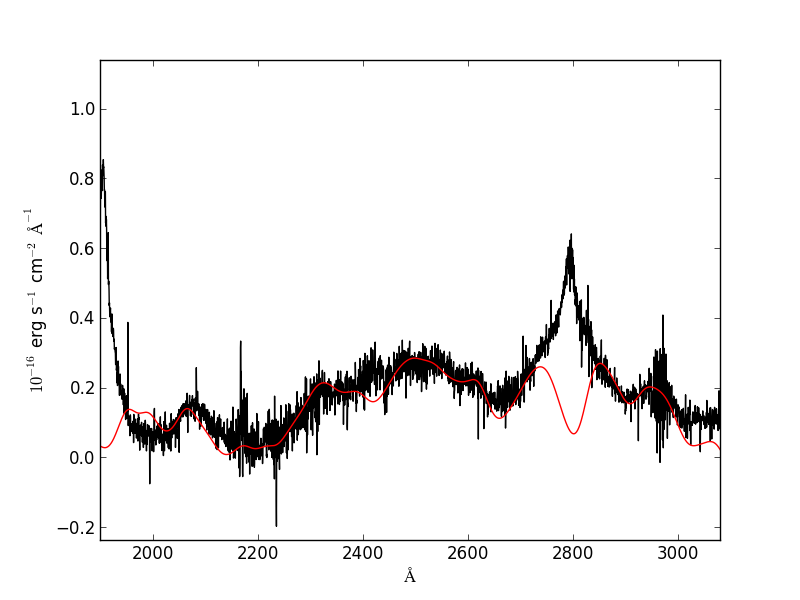
\includegraphics[width=0.49\linewidth,angle=0]{./full_range/fe_fit_SBB_2.png}
\hspace{5mm}
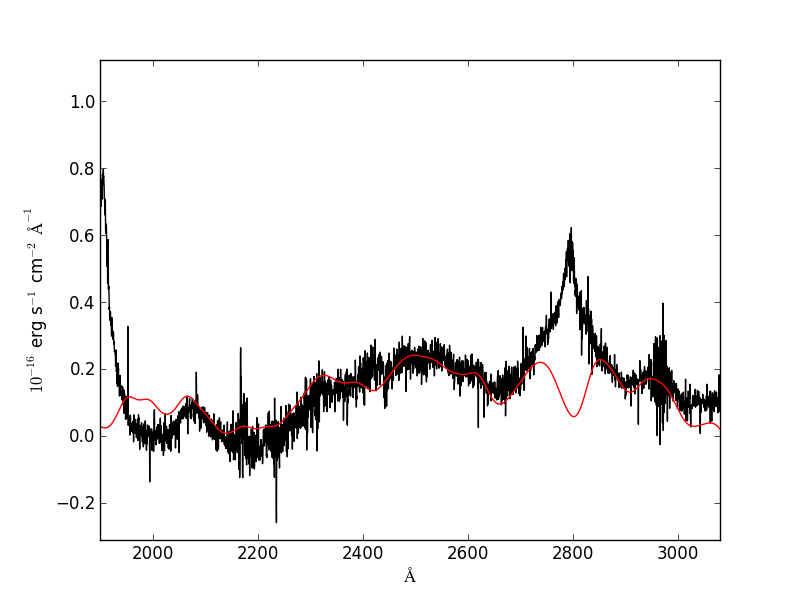
\includegraphics[width=0.46\linewidth,angle=0]{./Fe_fit_slope_break/fe_fit_SBB_2.png}\\
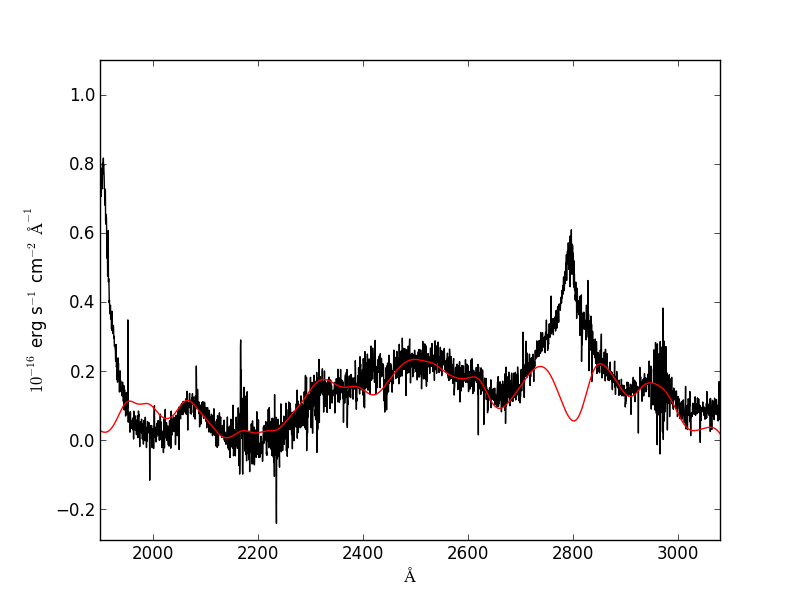
\includegraphics[width=0.46\linewidth,angle=0]{./Blue/fe_fit_SBB_2.png}
\vspace{5mm}
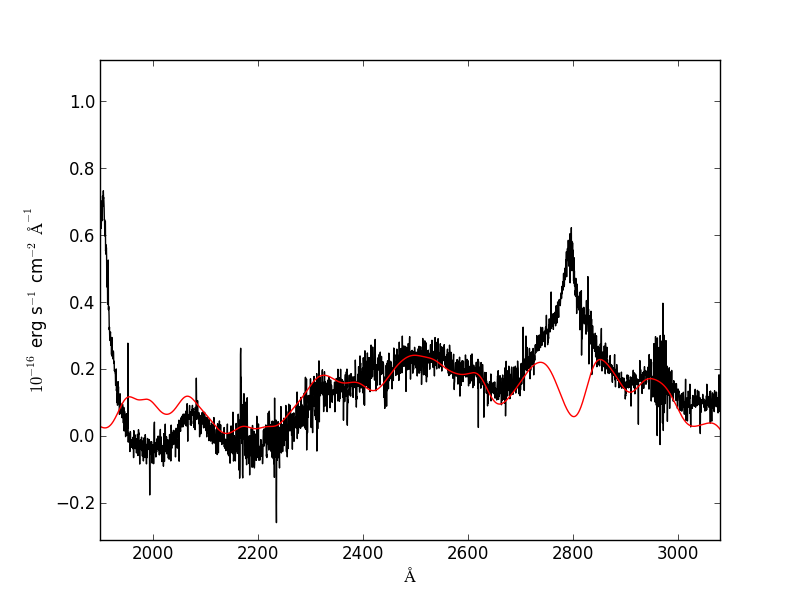
\includegraphics[width=0.49\linewidth,angle=0]{./red/fe_fit_SBB_2.png}\\

\end{center} 
\caption{J0941+0443 \label{fig:landscape}}   
\end{figure*}

\newpage

\begin{figure*}
\begin{center}
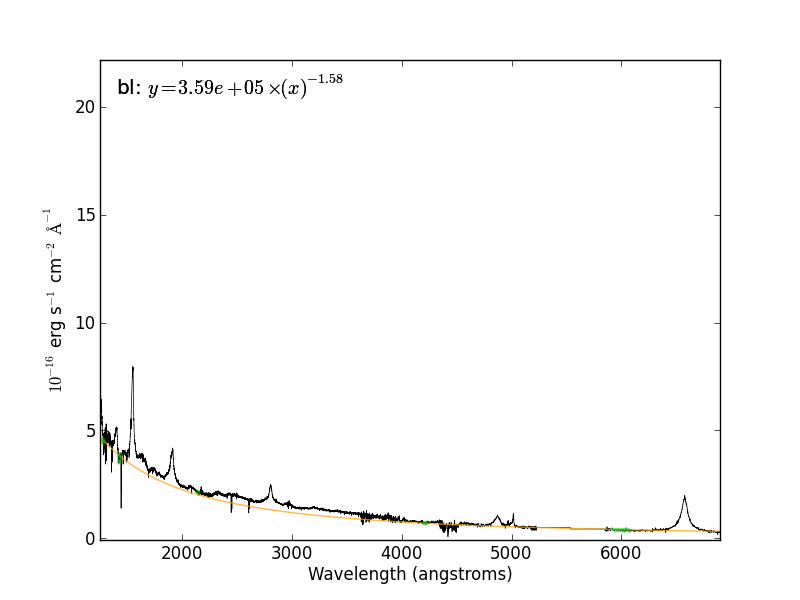
\includegraphics[width=0.49\linewidth,angle=0]{./full_range/continuous_3.png}
\vspace{5mm}
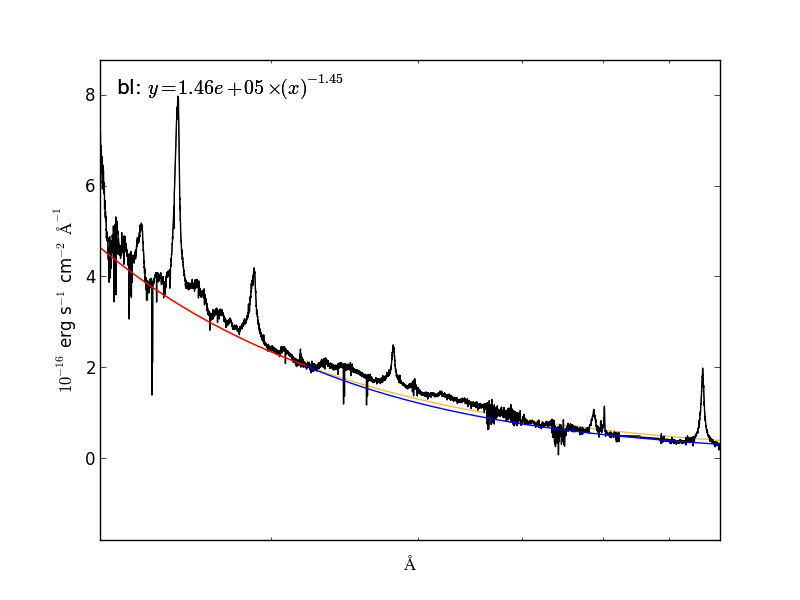
\includegraphics[width=0.46\linewidth,angle=0]{./Fe_fit_slope_break/break_continuous_3.png}\\
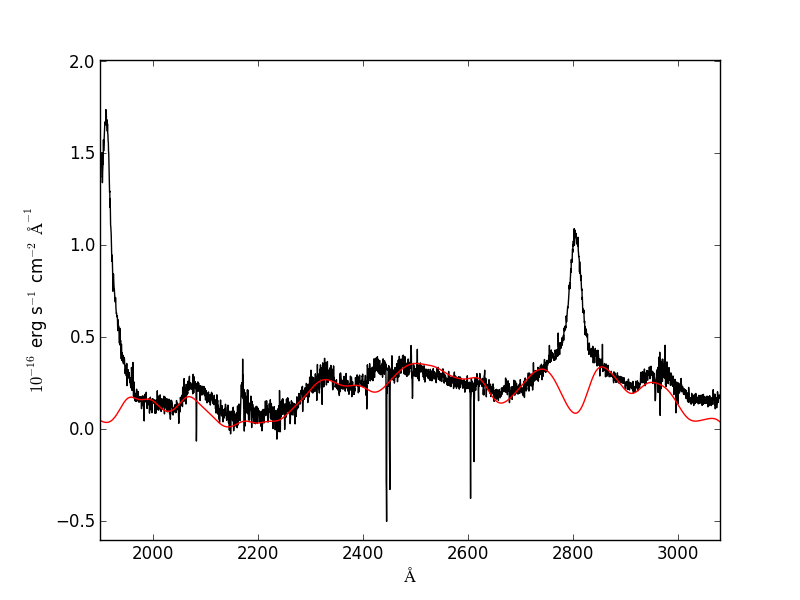
\includegraphics[width=0.49\linewidth,angle=0]{./full_range/fe_fit_SBB_3.png}
\hspace{5mm}
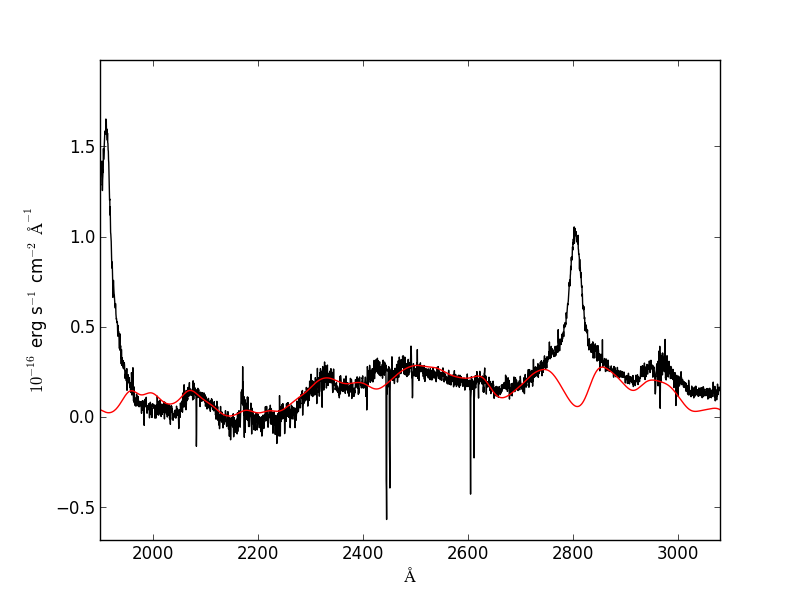
\includegraphics[width=0.46\linewidth,angle=0]{./Fe_fit_slope_break/fe_fit_SBB_3.png}\\
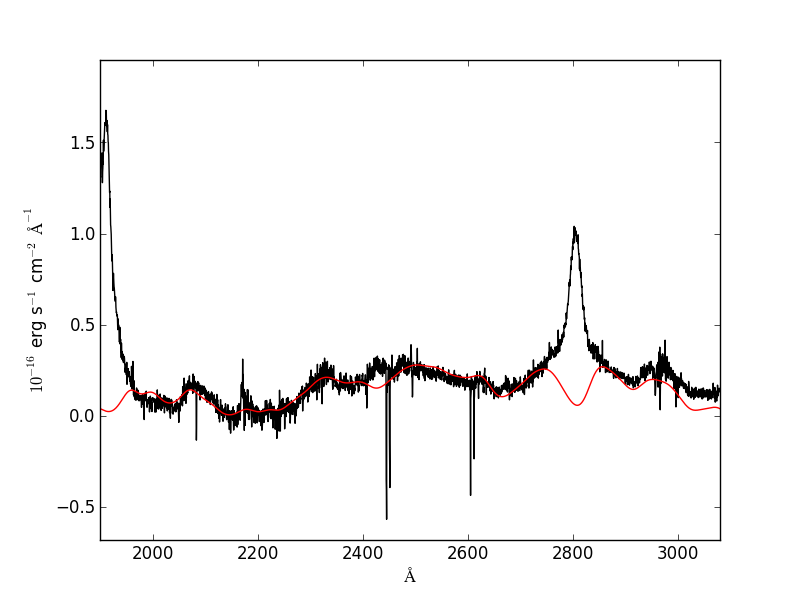
\includegraphics[width=0.46\linewidth,angle=0]{./Blue/fe_fit_SBB_3.png}
\vspace{5mm}
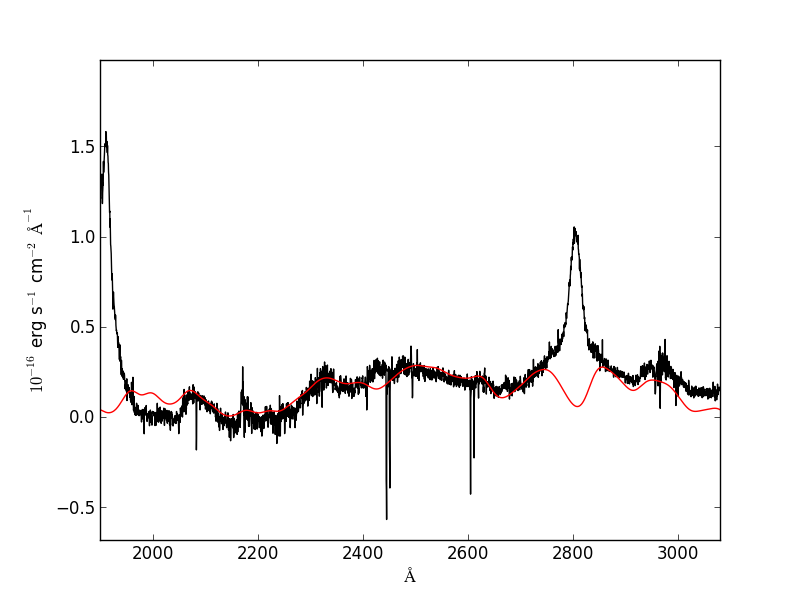
\includegraphics[width=0.49\linewidth,angle=0]{./red/fe_fit_SBB_3.png}\\

\end{center} 
\caption{J0209-0947 \label{fig:landscape}}   
\end{figure*}

\newpage



\begin{figure*}
\begin{center}
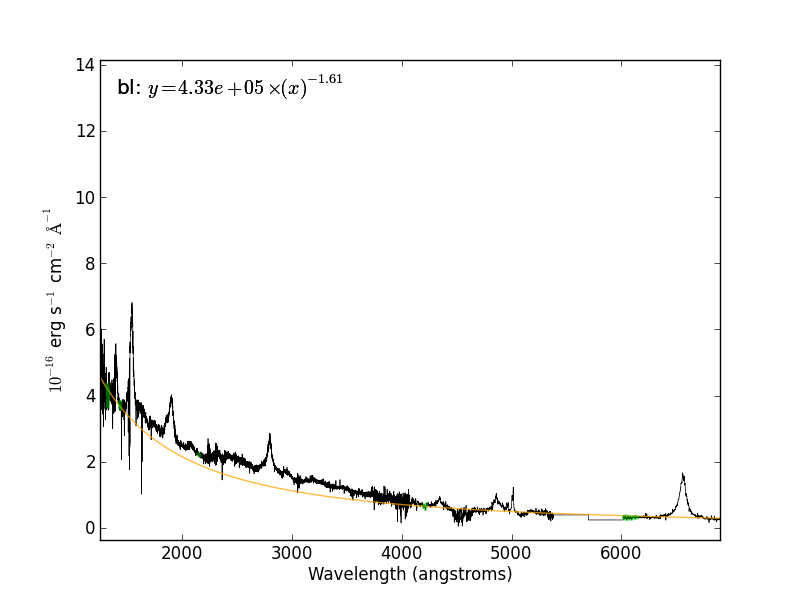
\includegraphics[width=0.49\linewidth,angle=0]{./full_range/continuous_5.png}
\vspace{5mm}
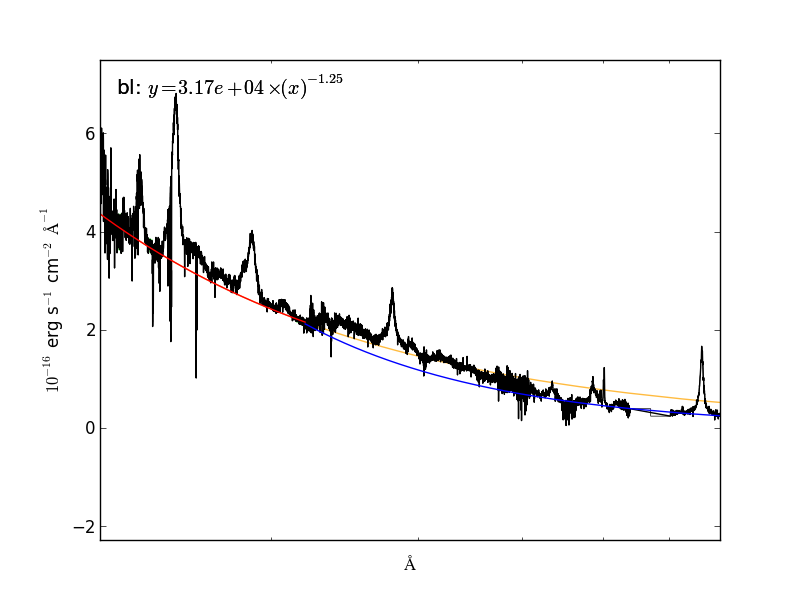
\includegraphics[width=0.46\linewidth,angle=0]{./Fe_fit_slope_break/break_continuous_5.png}\\
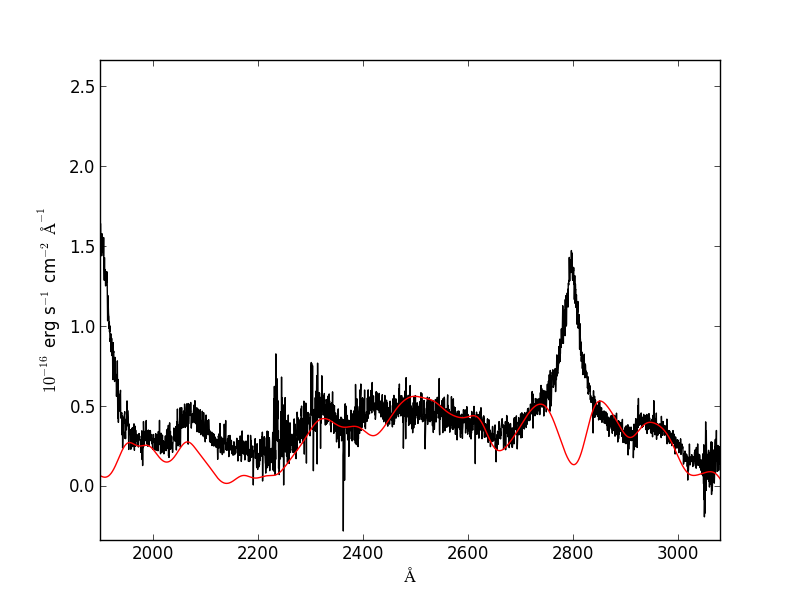
\includegraphics[width=0.49\linewidth,angle=0]{./full_range/fe_fit_SBB_5.png}
\hspace{5mm}
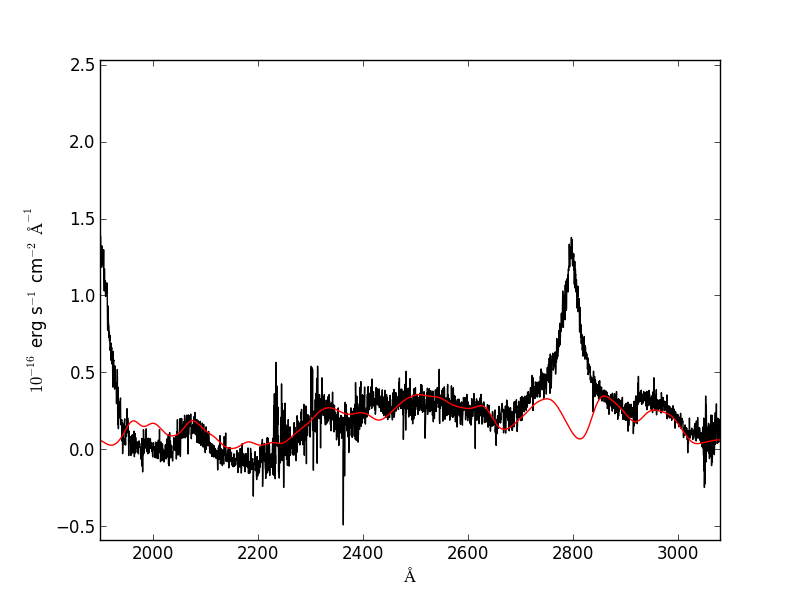
\includegraphics[width=0.46\linewidth,angle=0]{./Fe_fit_slope_break/fe_fit_SBB_5.png}\\
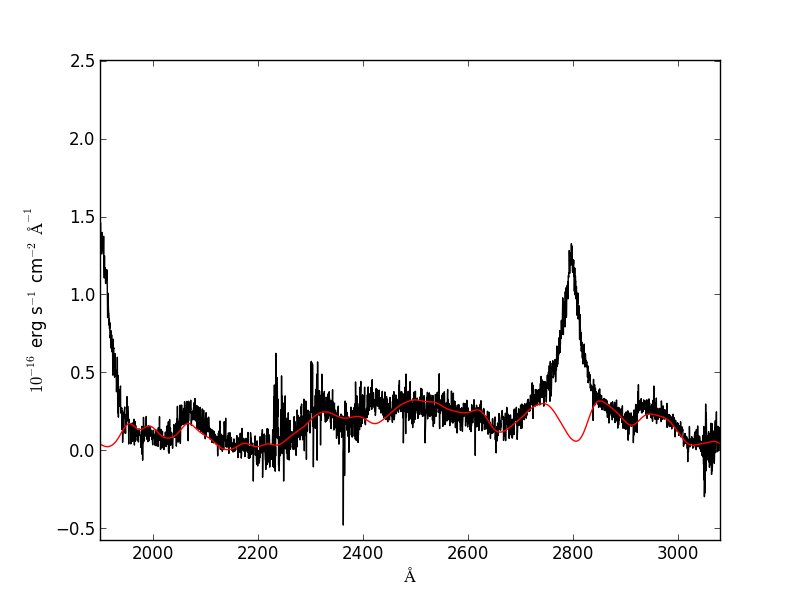
\includegraphics[width=0.46\linewidth,angle=0]{./Blue/fe_fit_SBB_5.png}
\vspace{5mm}
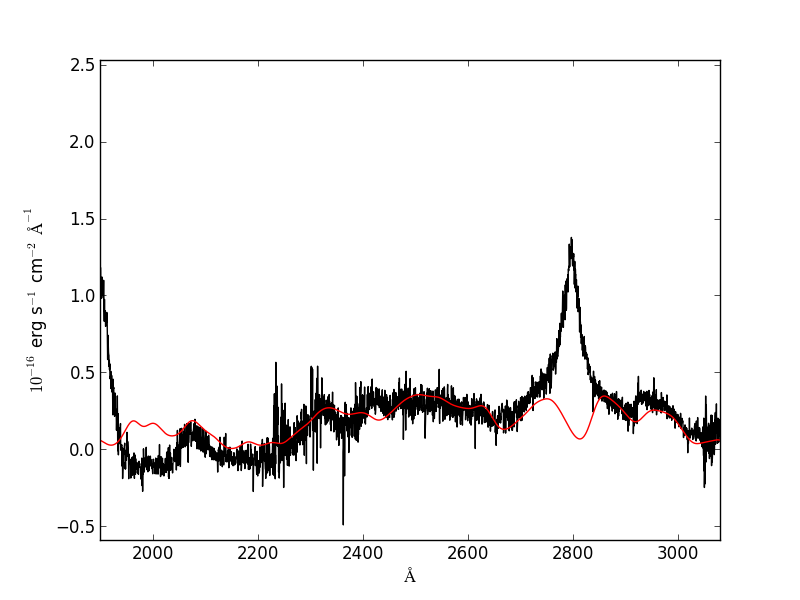
\includegraphics[width=0.49\linewidth,angle=0]{./red/fe_fit_SBB_5.png}\\

\end{center} 
\caption{J0842+0151 \label{fig:landscape}}   
\end{figure*}

\newpage

\begin{figure*}
\begin{center}
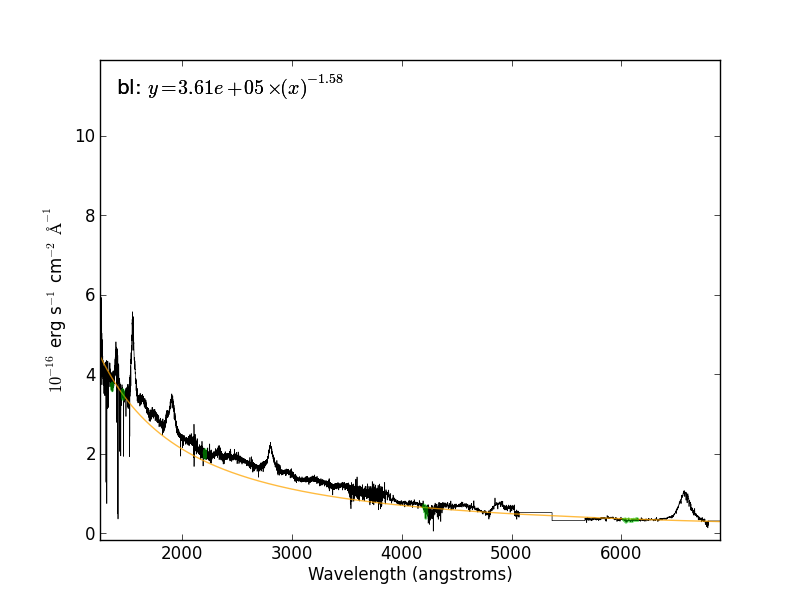
\includegraphics[width=0.49\linewidth,angle=0]{./full_range/continuous_6.png}
\vspace{5mm}
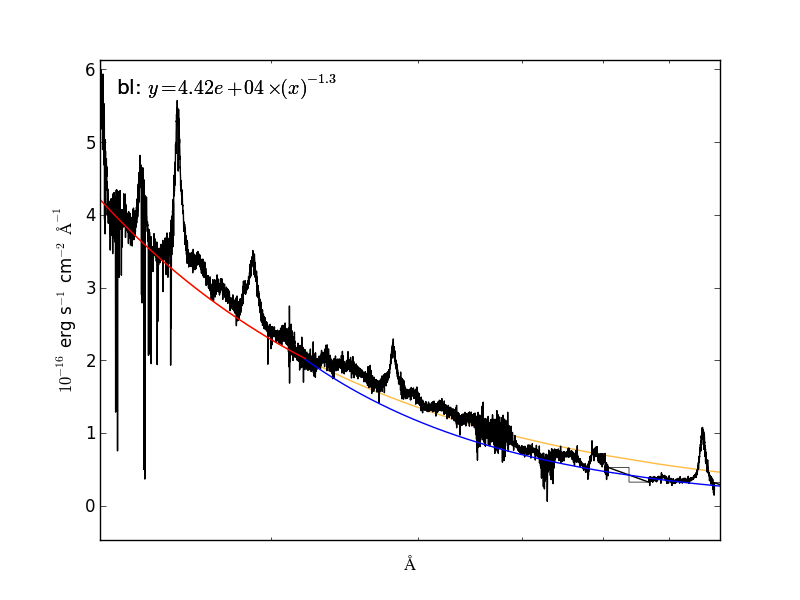
\includegraphics[width=0.46\linewidth,angle=0]{./Fe_fit_slope_break/break_continuous_6.png}\\
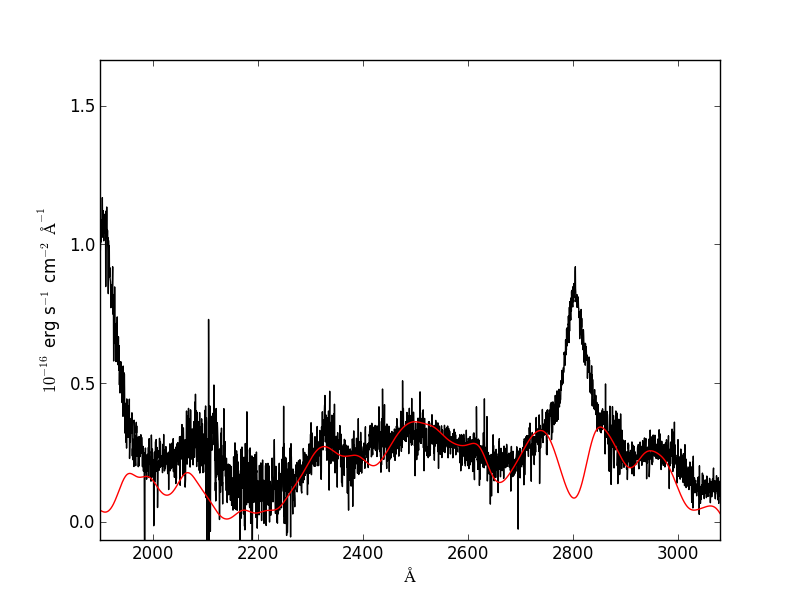
\includegraphics[width=0.49\linewidth,angle=0]{./full_range/fe_fit_SBB_6.png}
\hspace{5mm}
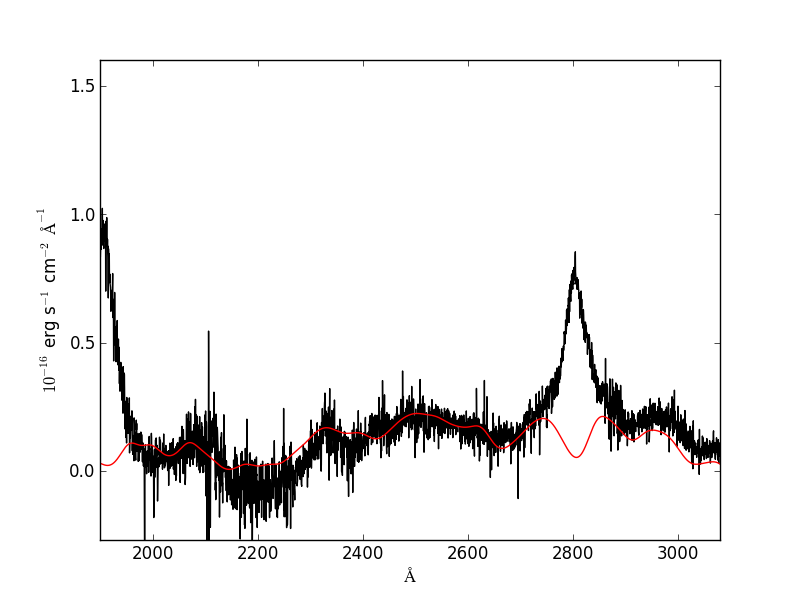
\includegraphics[width=0.46\linewidth,angle=0]{./Fe_fit_slope_break/fe_fit_SBB_6.png}\\
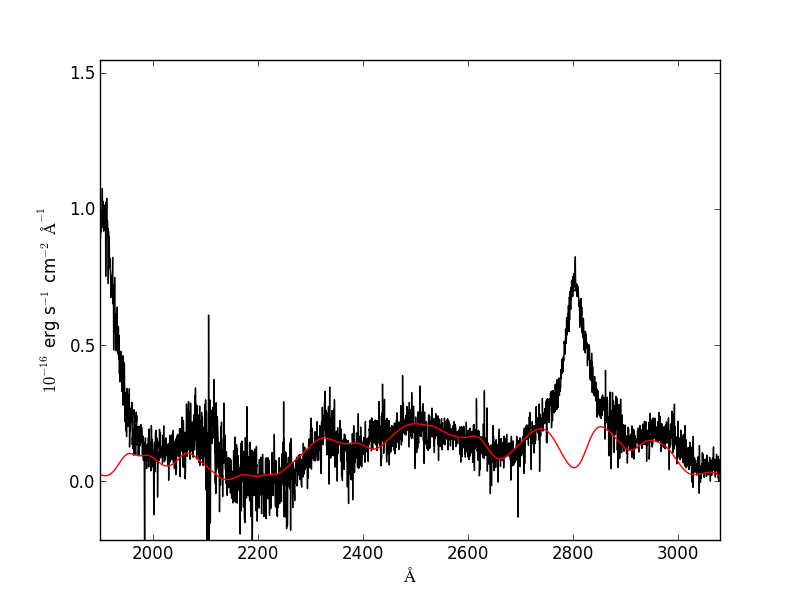
\includegraphics[width=0.46\linewidth,angle=0]{./Blue/fe_fit_SBB_6.png}
\vspace{5mm}
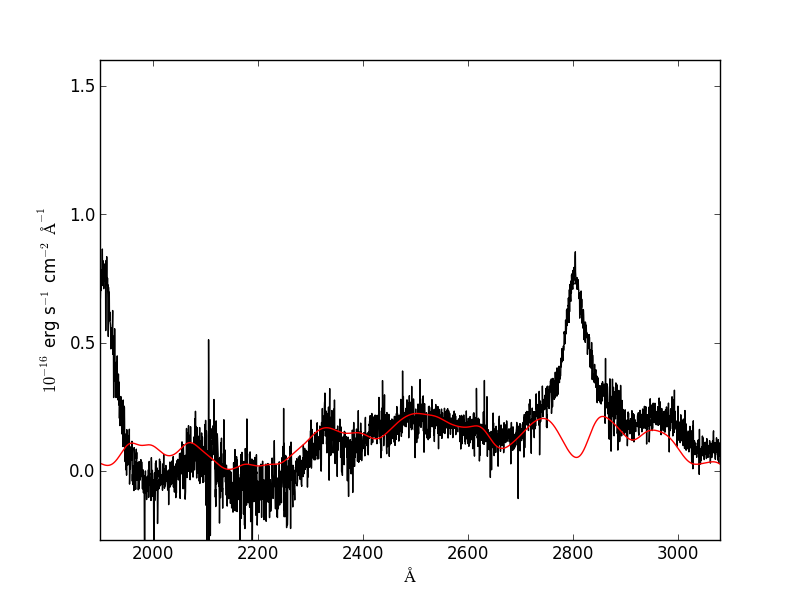
\includegraphics[width=0.49\linewidth,angle=0]{./red/fe_fit_SBB_6.png}\\

\end{center} 
\caption{J0303+0027 \label{fig:landscape}}   
\end{figure*}

\newpage

\begin{figure*}
\begin{center}
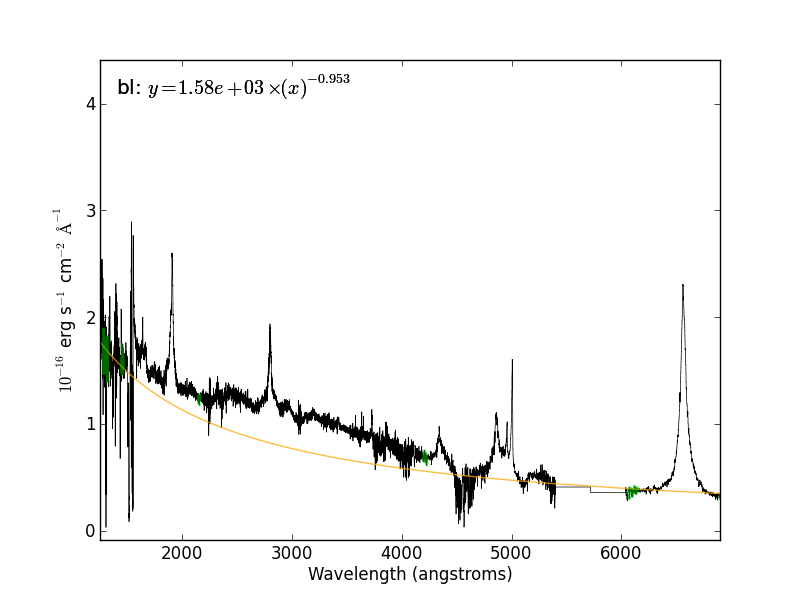
\includegraphics[width=0.49\linewidth,angle=0]{./full_range/continuous_7.png}
\vspace{5mm}
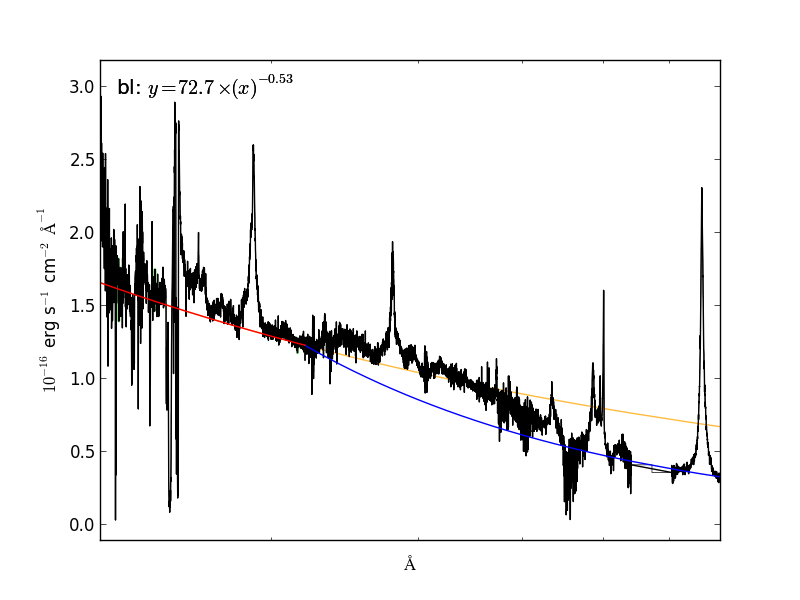
\includegraphics[width=0.46\linewidth,angle=0]{./Fe_fit_slope_break/break_continuous_7.png}\\
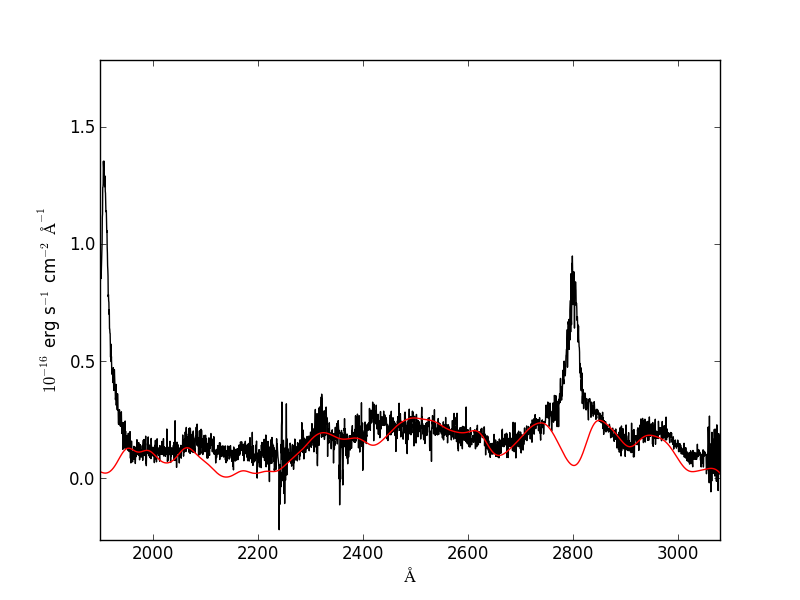
\includegraphics[width=0.49\linewidth,angle=0]{./full_range/fe_fit_SBB_7.png}
\hspace{5mm}
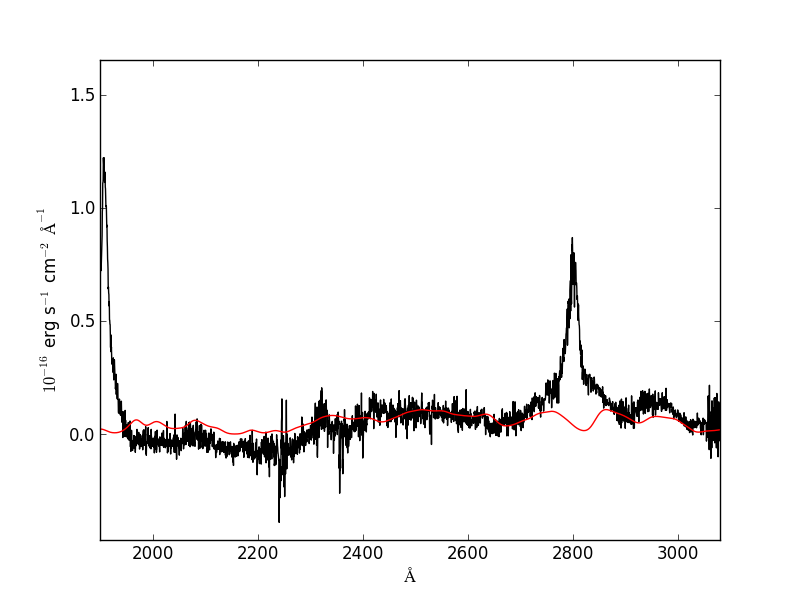
\includegraphics[width=0.46\linewidth,angle=0]{./Fe_fit_slope_break/fe_fit_SBB_7.png}\\
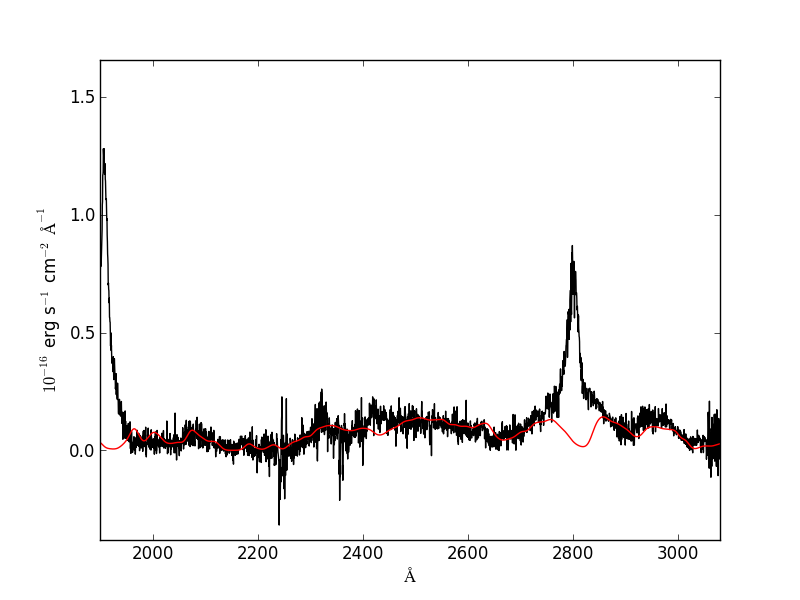
\includegraphics[width=0.46\linewidth,angle=0]{./Blue/fe_fit_SBB_7.png}
\vspace{5mm}
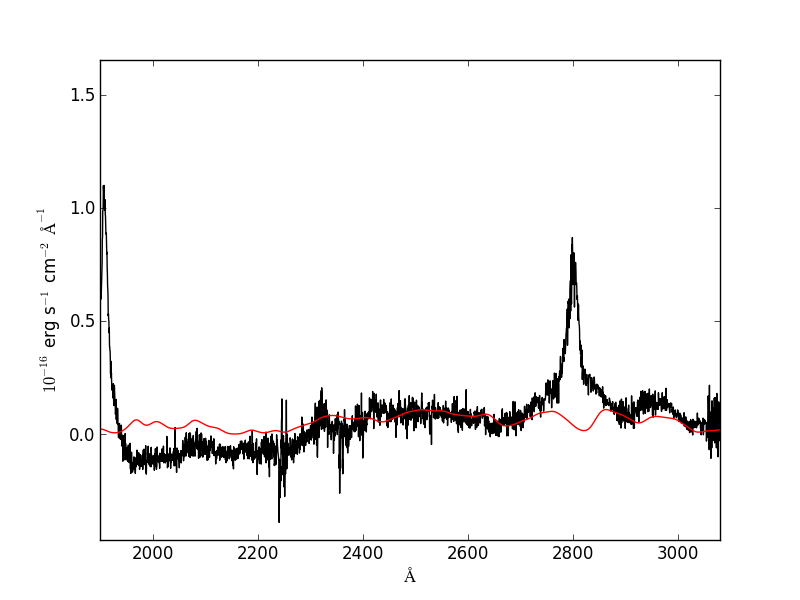
\includegraphics[width=0.49\linewidth,angle=0]{./red/fe_fit_SBB_7.png}\\

\end{center} 
\caption{J1005+0245 \label{fig:landscape}}   
\end{figure*}

\newpage

\begin{figure*}
\begin{center}
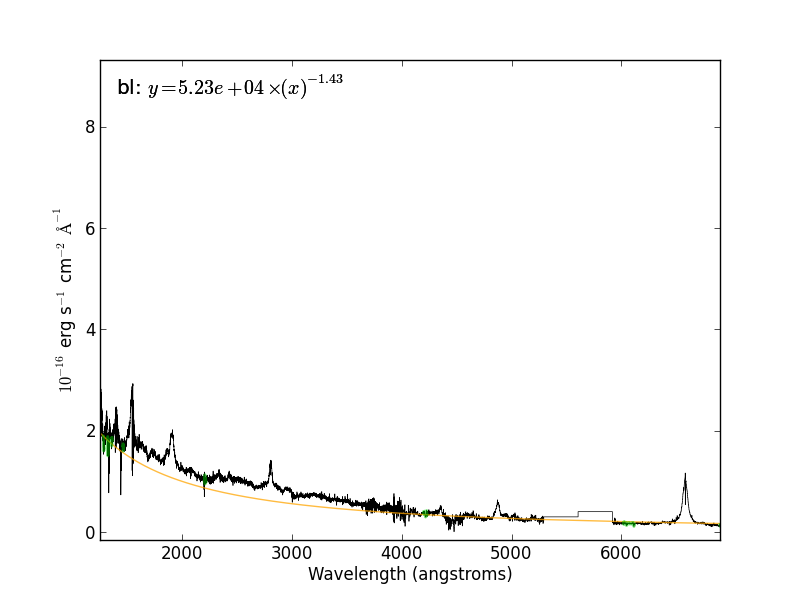
\includegraphics[width=0.49\linewidth,angle=0]{./full_range/continuous_8.png}
\vspace{5mm}
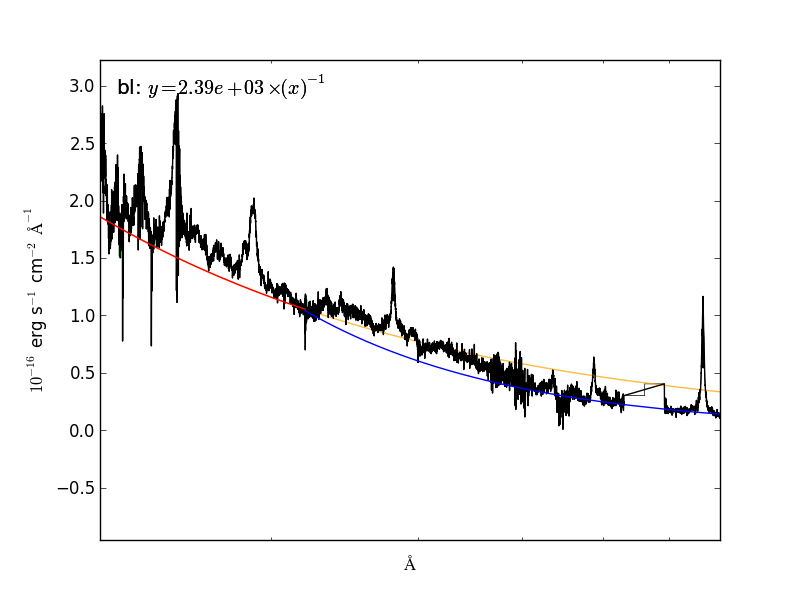
\includegraphics[width=0.46\linewidth,angle=0]{./Fe_fit_slope_break/break_continuous_8.png}\\
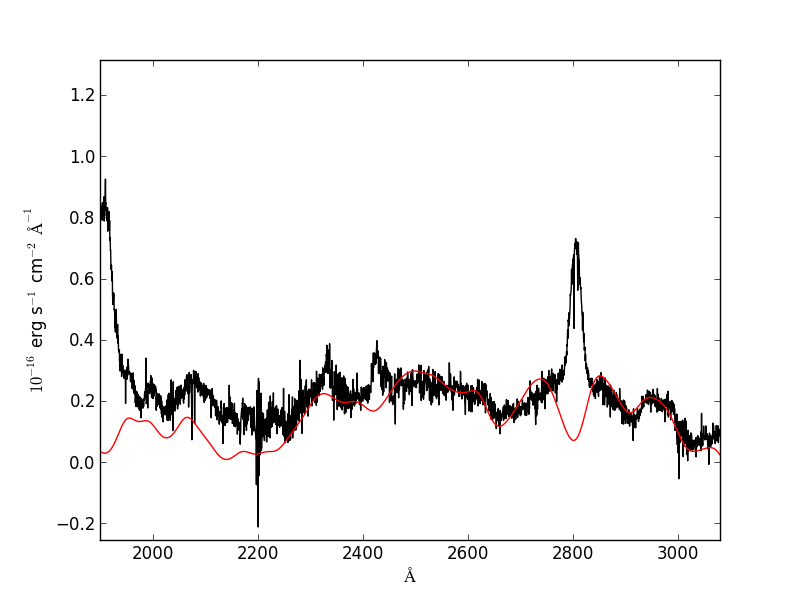
\includegraphics[width=0.49\linewidth,angle=0]{./full_range/fe_fit_SBB_8.png}
\hspace{5mm}
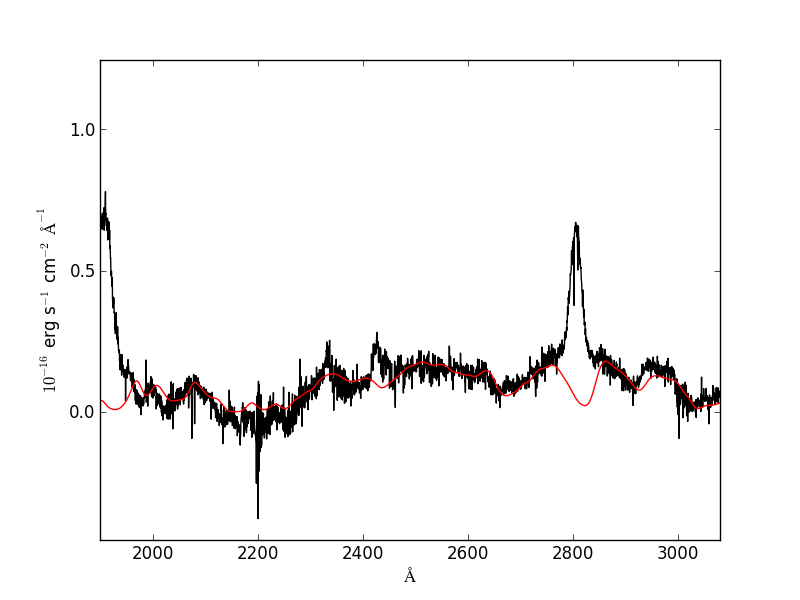
\includegraphics[width=0.46\linewidth,angle=0]{./Fe_fit_slope_break/fe_fit_SBB_8.png}\\
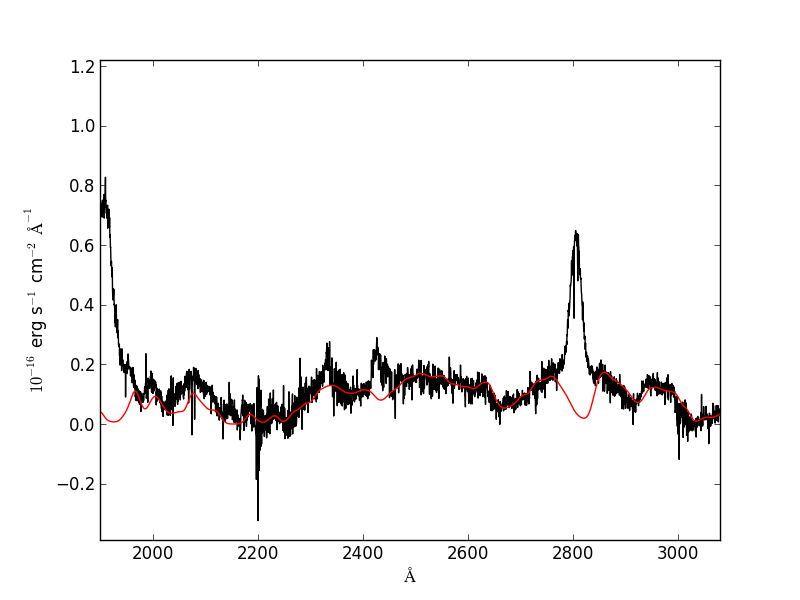
\includegraphics[width=0.46\linewidth,angle=0]{./Blue/fe_fit_SBB_8.png}
\vspace{5mm}
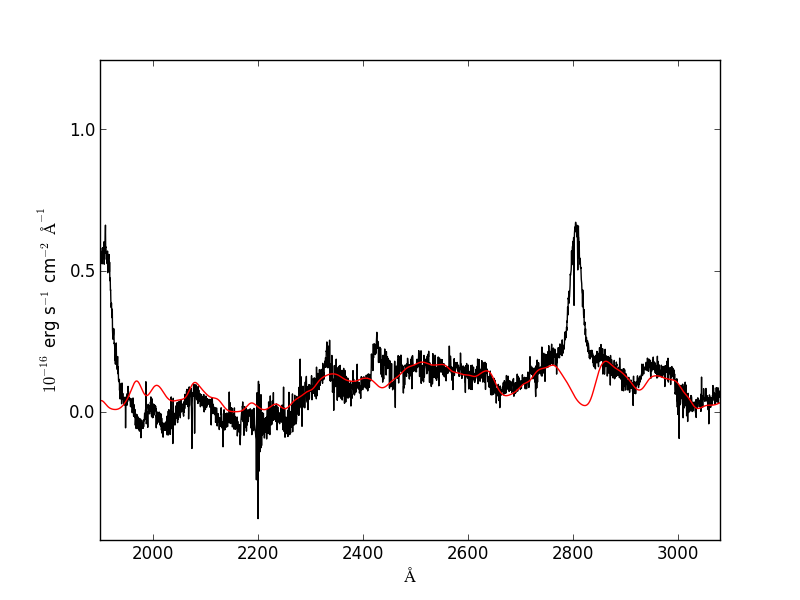
\includegraphics[width=0.49\linewidth,angle=0]{./red/fe_fit_SBB_8.png}\\

\end{center} 
\caption{J0934+0005 \label{fig:landscape}}   
\end{figure*}

\newpage


\begin{figure*}
\begin{center}
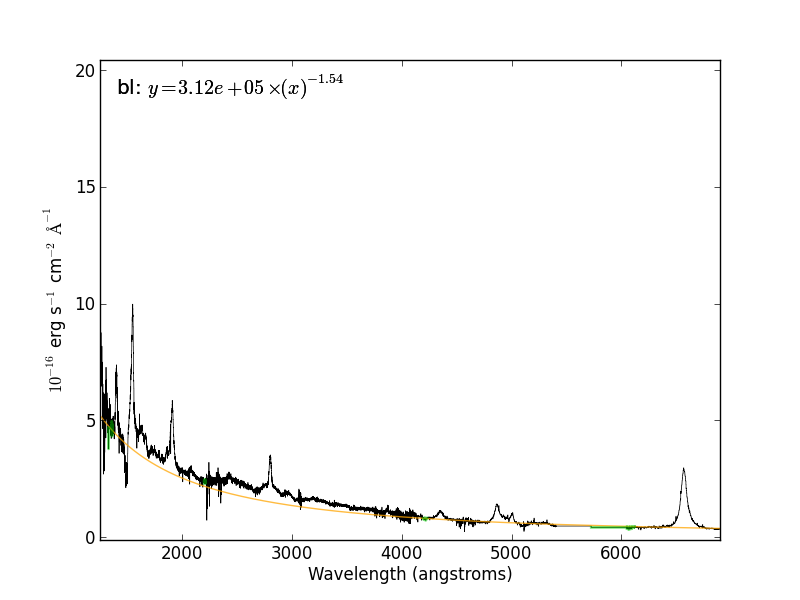
\includegraphics[width=0.49\linewidth,angle=0]{./full_range/continuous_9.png}
\vspace{5mm}
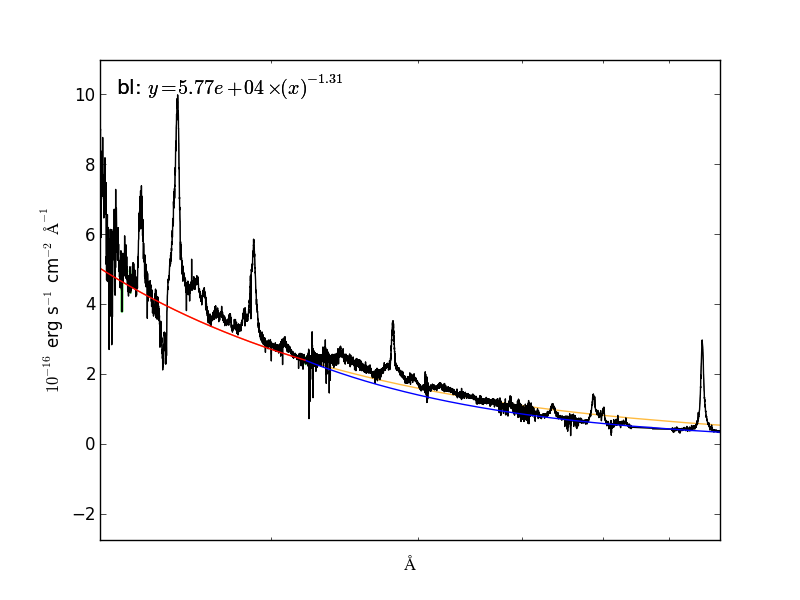
\includegraphics[width=0.46\linewidth,angle=0]{./Fe_fit_slope_break/break_continuous_9.png}\\
\includegraphics[width=0.49\linewidth,angle=0]{./full_range/fe_fit_SBB_9.png}
\hspace{5mm}
\includegraphics[width=0.46\linewidth,angle=0]{./Fe_fit_slope_break/fe_fit_SBB_9.png}\\
\includegraphics[width=0.46\linewidth,angle=0]{./Blue/fe_fit_SBB_9.png}
\vspace{5mm}
\includegraphics[width=0.49\linewidth,angle=0]{./red/fe_fit_SBB_9.png}\\

\end{center} 
\caption{J1002+0331 \label{fig:landscape}}   
\end{figure*}

\newpage

\begin{figure*}
\begin{center}
\includegraphics[width=0.49\linewidth,angle=0]{./full_range/continuous_10.png}
\vspace{5mm}
\includegraphics[width=0.46\linewidth,angle=0]{./Fe_fit_slope_break/break_continuous_10.png}\\
\includegraphics[width=0.49\linewidth,angle=0]{./full_range/fe_fit_SBB_10.png}
\hspace{5mm}
\includegraphics[width=0.46\linewidth,angle=0]{./Fe_fit_slope_break/fe_fit_SBB_10.png}\\
\includegraphics[width=0.46\linewidth,angle=0]{./Blue/fe_fit_SBB_10.png}
\vspace{5mm}
\includegraphics[width=0.49\linewidth,angle=0]{./red/fe_fit_SBB_10.png}\\

\end{center} 
\caption{J0323-0029 \label{fig:landscape}}   
\end{figure*}

\newpage

\begin{figure*}
\begin{center}
\includegraphics[width=0.49\linewidth,angle=0]{./full_range/continuous_11.png}
\vspace{5mm}
\includegraphics[width=0.46\linewidth,angle=0]{./Fe_fit_slope_break/break_continuous_11.png}\\
\includegraphics[width=0.49\linewidth,angle=0]{./full_range/fe_fit_SBB_11.png}
\hspace{5mm}
\includegraphics[width=0.46\linewidth,angle=0]{./Fe_fit_slope_break/fe_fit_SBB_11.png}\\
\includegraphics[width=0.46\linewidth,angle=0]{./Blue/fe_fit_SBB_11.png}
\vspace{5mm}
\includegraphics[width=0.49\linewidth,angle=0]{./red/fe_fit_SBB_11.png}\\

\end{center} 
\caption{J1013+0245 \label{fig:landscape}}   
\end{figure*}

\newpage


\begin{figure*}
\begin{center}
\includegraphics[width=0.49\linewidth,angle=0]{./full_range/continuous_12.png}
\vspace{5mm}
\includegraphics[width=0.46\linewidth,angle=0]{./Fe_fit_slope_break/break_continuous_12.png}\\
\includegraphics[width=0.49\linewidth,angle=0]{./full_range/fe_fit_SBB_12.png}
\hspace{5mm}
\includegraphics[width=0.46\linewidth,angle=0]{./Fe_fit_slope_break/fe_fit_SBB_12.png}\\
\includegraphics[width=0.46\linewidth,angle=0]{./Blue/fe_fit_SBB_12.png}
\vspace{5mm}
\includegraphics[width=0.49\linewidth,angle=0]{./red/fe_fit_SBB_12.png}\\

\end{center} 
\caption{J0019-1053 \label{fig:landscape}}   
\end{figure*}

\newpage

\begin{figure*}
\begin{center}
\includegraphics[width=0.49\linewidth,angle=0]{./full_range/continuous_13.png}
\vspace{5mm}
\includegraphics[width=0.46\linewidth,angle=0]{./Fe_fit_slope_break/break_continuous_13.png}\\
\includegraphics[width=0.49\linewidth,angle=0]{./full_range/fe_fit_SBB_13.png}
\hspace{5mm}
\includegraphics[width=0.46\linewidth,angle=0]{./Fe_fit_slope_break/fe_fit_SBB_13.png}\\
\includegraphics[width=0.46\linewidth,angle=0]{./Blue/fe_fit_SBB_13.png}
\vspace{5mm}
\includegraphics[width=0.49\linewidth,angle=0]{./red/fe_fit_SBB_13.png}\\

\end{center} 
\caption{J0136-0015\label{fig:landscape}}   
\end{figure*}

\newpage


\begin{figure*}
\begin{center}
\includegraphics[width=0.49\linewidth,angle=0]{./full_range/continuous_14.png}
\vspace{5mm}
\includegraphics[width=0.46\linewidth,angle=0]{./Fe_fit_slope_break/break_continuous_14.png}\\
\includegraphics[width=0.49\linewidth,angle=0]{./full_range/fe_fit_SBB_14.png}
\hspace{5mm}
\includegraphics[width=0.46\linewidth,angle=0]{./Fe_fit_slope_break/fe_fit_SBB_14.png}\\
\includegraphics[width=0.46\linewidth,angle=0]{./Blue/fe_fit_SBB_14.png}
\vspace{5mm}
\includegraphics[width=0.49\linewidth,angle=0]{./red/fe_fit_SBB_14.png}\\

\end{center} 
\caption{J0223-0007 \label{fig:landscape}}   
\end{figure*}

\newpage


\begin{figure*}
\begin{center}
\includegraphics[width=0.49\linewidth,angle=0]{./full_range/continuous_15.png}
\vspace{5mm}
\includegraphics[width=0.46\linewidth,angle=0]{./Fe_fit_slope_break/break_continuous_15.png}\\
\includegraphics[width=0.49\linewidth,angle=0]{./full_range/fe_fit_SBB_15.png}
\hspace{5mm}
\includegraphics[width=0.46\linewidth,angle=0]{./Fe_fit_slope_break/fe_fit_SBB_15.png}\\
\includegraphics[width=0.46\linewidth,angle=0]{./Blue/fe_fit_SBB_15.png}
\vspace{5mm}
\includegraphics[width=0.49\linewidth,angle=0]{./red/fe_fit_SBB_15.png}\\

\end{center} 
\caption{J0948+0137 \label{fig:landscape}}   
\end{figure*}


\end{document}
